%====================================================================
% CS6007 Project: findings so far in the decentralised setting
% Decentralised Single-Index Bandits (Paper A, branch Dec-SIB)
% Template originally from the first pitch deck (slides/pitch, in git history). Update the "Next steps" and
% "Status" slides as new work lands.
%====================================================================
\documentclass[11pt]{beamer}
\usetheme{Madrid}
\usecolortheme{beaver}
\usefonttheme{professionalfonts}
\usepackage[T1]{fontenc}
\usepackage[utf8]{inputenc}
\usepackage{lmodern}
\usepackage{amsmath,amssymb,amsthm}
\usepackage{graphicx}
\usepackage{hyperref}
\usepackage{tikz}
\usetikzlibrary{arrows,positioning,shapes,patterns}
\usepackage{booktabs}
\usepackage{array}
\usepackage{pifont}

\graphicspath{{figs/}}
\setbeamertemplate{navigation symbols}{}
\setbeamerfont{footnote}{size=\tiny}
\newcommand{\yes}{\textcolor{green!45!black}{\ding{51}}}
\newcommand{\no}{\textcolor{red!70!black}{\ding{55}}}
\newcommand{\todo}{\textcolor{orange!85!black}{\ding{109}}}

\title[Decentralised Single-Index Bandits]{Decentralised Single-Index Bandits}
\subtitle{Backup slides: proofs, extra experiments and earlier findings}
\author[Harshitha \& Nischal]{\texorpdfstring{\textbf{Presented by:}\\[0.3em]\begin{tabular}{rl}\textcolor{blue}{Harshitha (23b1071)} & Dept. of CSE\\\textcolor{blue}{Nischal (23b1024)} & Dept. of CSE\end{tabular}\\[0.8em]\textbf{Course:} CS6007: Multi-Agent Machine Learning\\[0.2em]\textbf{Instructor:} Prof.\ Avishek Ghosh}{Harshitha, Nischal}}
\institute[IIT Bombay]{IIT Bombay}
\date{\small 25 October 2026}

\addtobeamertemplate{frametitle}{}{%
\begin{tikzpicture}[remember picture,overlay]
\node[anchor=north east,xshift=0.2cm,yshift=0.4cm] at (current page.north east){
\includegraphics[height=1.1cm]{iitb_logo.png}};
\end{tikzpicture}}

\begin{document}

\usebackgroundtemplate{\tikz[remember picture,overlay]\node[opacity=0.15] at ([yshift=-2cm]current page.center){
\includegraphics[width=0.6\paperwidth]{iitb_logo.png}};}
\begin{frame}\titlepage\end{frame}
\usebackgroundtemplate{}



%====================================================================
\begin{frame}{The flood relay used in the early experiments}
\small
\begin{block}{Phase 1: exact pooling without a server}
Stein sums are \textbf{sufficient statistics}: spanning-tree aggregation (up and back down a BFS tree, $2\cdot$depth rounds) gives \emph{every} agent the exact centralised $\hat\theta$.
\end{block}
\begin{block}{Freeze: one shared grid}
All agents freeze the same $\hat\theta$; the window $W$ comes from max-consensus over $D$ rounds.
\end{block}
\begin{block}{Phase 2: event-triggered flooding of bin tables}
Each agent stores the freshest copy of every agent's own $(n_j,S_j)$ table, relayed one hop per round. An agent republishes only when its unpublished count in a bin exceeds $\gamma\times$ what it currently sees.
\end{block}
\begin{alertblock}{Design principle}
\centering \textbf{Relay exact, sparse updates instead of averaging.}
\end{alertblock}
\end{frame}

%====================================================================
\begin{frame}{The version we analyse: synchronised epochs}
\small
\begin{block}{Phase 2, as analysed ($\Lambda$ = delivery time, $=D$ on a static graph)}
\begin{itemize}
\item Every $L=2\Lambda$ rounds, an agent raises an \textbf{alarm} if its own new pulls in some bin exceed $\gamma\times$ the network count at the last epoch. Any alarm $\Rightarrow$ an \textbf{epoch}.
\item At an epoch every agent floods a \textbf{snapshot} of the bins it pulled since the last one.
\item Every agent acts on the \textbf{same} epoch table $G(e)$ plus its \textbf{own} pulls since $e$.
\end{itemize}
\end{block}
\begin{center}
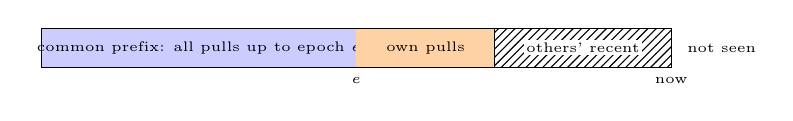
\begin{tikzpicture}[x=0.8cm,y=0.5cm,font=\tiny]
\fill[blue!20] (0,0) rectangle (5,1); \node at (2.5,0.5) {common prefix: all pulls up to epoch $e$};
\fill[orange!35] (5,0) rectangle (7.2,1); \node at (6.1,0.5) {own pulls};
\draw[pattern=north east lines] (7.2,0) rectangle (10,1); \node[fill=white,inner sep=1pt] at (8.6,0.5) {others' recent};
\draw (0,0) rectangle (10,1);
\node[anchor=north] at (5,0) {$e$}; \node[anchor=north] at (10,0) {now};
\node[anchor=west] at (10.1,0.5) {not seen};
\end{tikzpicture}
\end{center}
\begin{alertblock}{Why this version}
What an agent sees is \emph{one common prefix plus one own block}, so the confidence width is exactly the server's. In the code version each agent sees $N$ separate per-agent prefixes, and the proof loses a factor $\sqrt N$.
\end{alertblock}
\end{frame}

%====================================================================
\begin{frame}{E31: the protocol we prove vs the protocol we run}
\scriptsize
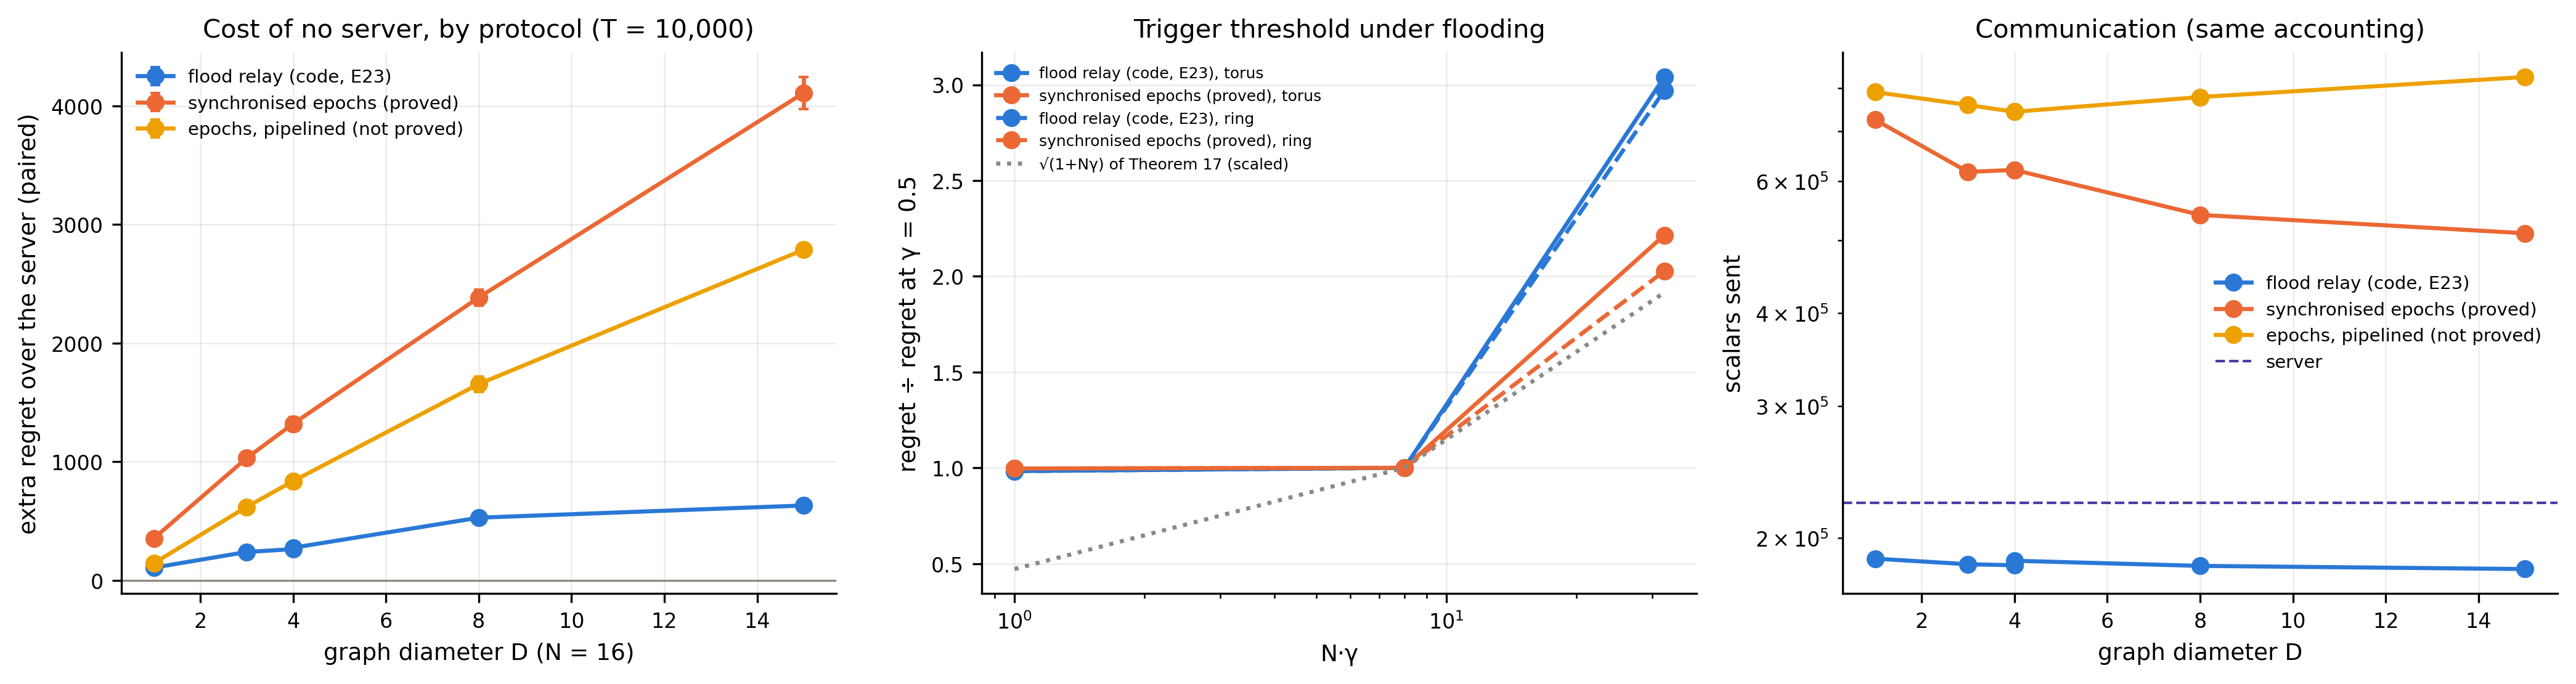
\includegraphics[width=0.86\textwidth]{e31_epoch.png}
\begin{columns}[T]
\begin{column}{0.5\textwidth}
\begin{itemize}
\item \textbf{Proved (synchronised epochs):} $+5\%$ ($D{=}1$) to $+59\%$ ($D{=}15$) over the server; grows like $D^{0.9}$.
\item \textbf{Run (flood relay):} $+1.5\%$ to $+9\%$; grows like $D^{0.66}$.
\item Pipelined epochs (not proved): a third of the gap.
\end{itemize}
\end{column}
\begin{column}{0.48\textwidth}
\begin{itemize}
\item \textbf{Trigger:} $\gamma\le0.5$ is free for both ($\le2\%$); only $\gamma=2$ costs ($\times2$--$3$).
\item \textbf{Scalars:} epochs send $2.4$--$3.8\times$ more (every agent snapshots at every epoch).
\end{itemize}
\end{column}
\end{columns}
\vspace{0.2em}
\begin{alertblock}{Why: agreement costs latency}
To use a common table, every agent waits for the \emph{farthest} agent ($\approx4D$ rounds). The relay uses nearby agents' pulls after a few hops. \textbf{Closed by Theorem 27:} the published-only relay is provable and performs like the relay (E36).
\end{alertblock}
\end{frame}

%====================================================================
\begin{frame}{Mixing vs relaying: building a network sum}
\footnotesize
Every agent needs network totals: $\sum_i b_i$ (Phase 1) and $n_j,S_j$ per bin (Phase 2).
Toy example: ring of 4 agents with values $(4,0,0,0)$; true average $=1$.
\begin{columns}[T]
\begin{column}{0.49\textwidth}
\begin{block}{Mixing (consensus / gossip)}
Each round: $x_i\leftarrow\sum_j P_{ij}x_j$ \;(average with neighbours)\\[0.3em]
\scriptsize
\begin{tabular}{ccccc}
\toprule
round & $a_1$ & $a_2$ & $a_3$ & $a_4$\\
\midrule
0 & 4 & 0 & 0 & 0\\
1 & 1.33 & 1.33 & 0 & 1.33\\
2 & 1.33 & 0.89 & 0.89 & 0.89\\
3 & 1.04 & 1.04 & 0.89 & 1.04\\
\bottomrule
\end{tabular}\\[0.2em]
$\to1$ but \textbf{never exact}; speed set by the \emph{spectral gap}. Sends the whole state every round.
\end{block}
\end{column}
\begin{column}{0.49\textwidth}
\begin{block}{Relaying (flooding / message passing)}
Each round: forward fresher copies of \emph{each agent's own} record (with a version stamp).\\[0.3em]
\scriptsize
\begin{tabular}{cl}
\toprule
round & who knows ``$a_1$ has 4''\\
\midrule
1 & $a_2$, $a_4$\\
2 & everyone\\
\bottomrule
\end{tabular}\\[0.2em]
\textbf{Exact} after $D$ rounds (diameter); sends only records that changed.
\end{block}
\end{column}
\end{columns}
\vspace{0.1em}
\centering UCB uses counts directly ($1/\sqrt{n_j}$): mixing gives \emph{approximate} counts, relaying gives \emph{exact but stale} ones.
\end{frame}

%====================================================================
\begin{frame}{When does relaying win? Scope and limitations}
\scriptsize
\begin{block}{Our claim (not ``relaying beats mixing'' in general)}
For nonparametric bandits whose sufficient statistic is a \textbf{sparse table} (bin counts and sums), relaying exact, event-triggered updates \textbf{matches the regret} of consensus-based protocols with \textbf{orders of magnitude fewer scalars}, and is more robust to sparse or unreliable graphs.
\end{block}
\begin{columns}[T]
\begin{column}{0.5\textwidth}
\begin{alertblock}{Limitations of the flood relay (code)}
\begin{itemize}
\item Memory $O(N\cdot N_{\mathrm{bins}})$ per agent
\item Agents need unique IDs (no double counting)
\item Individual agents' statistics are shared
\end{itemize}
\end{alertblock}
\end{column}
\begin{column}{0.48\textwidth}
\begin{block}{What the epoch protocol fixes (Prop 30)}
\begin{itemize}
\item \textbf{Memory $O(N_{\mathrm{bins}}+N)$:} keep only the summed table
\item \textbf{Tree version:} $O(N_{\mathrm{bins}})$, no global IDs, only subtree partial sums are seen
\item \textbf{Privacy:} Phase 1 provably private (Thm 35), but costly; Phase 2 open
\end{itemize}
\end{block}
\end{column}
\end{columns}
\vspace{0.1em}
\scriptsize
\textbf{Why most papers mix:} constant memory in $N$, anonymous agents, built-in blending of data, a mature spectral-gap toolkit, and communication counted in \emph{rounds}, where both cost one message per edge.
\textbf{Precedent for relaying:} Dubey \& Pentland (Coop-KernelUCB) use message passing for the same reason: averaging biases the estimates.
\end{frame}

%====================================================================
\begin{frame}{Reference: a server $=$ one agent with $NT$ pulls}
\small
\begin{columns}[c]
\begin{column}{0.5\textwidth}
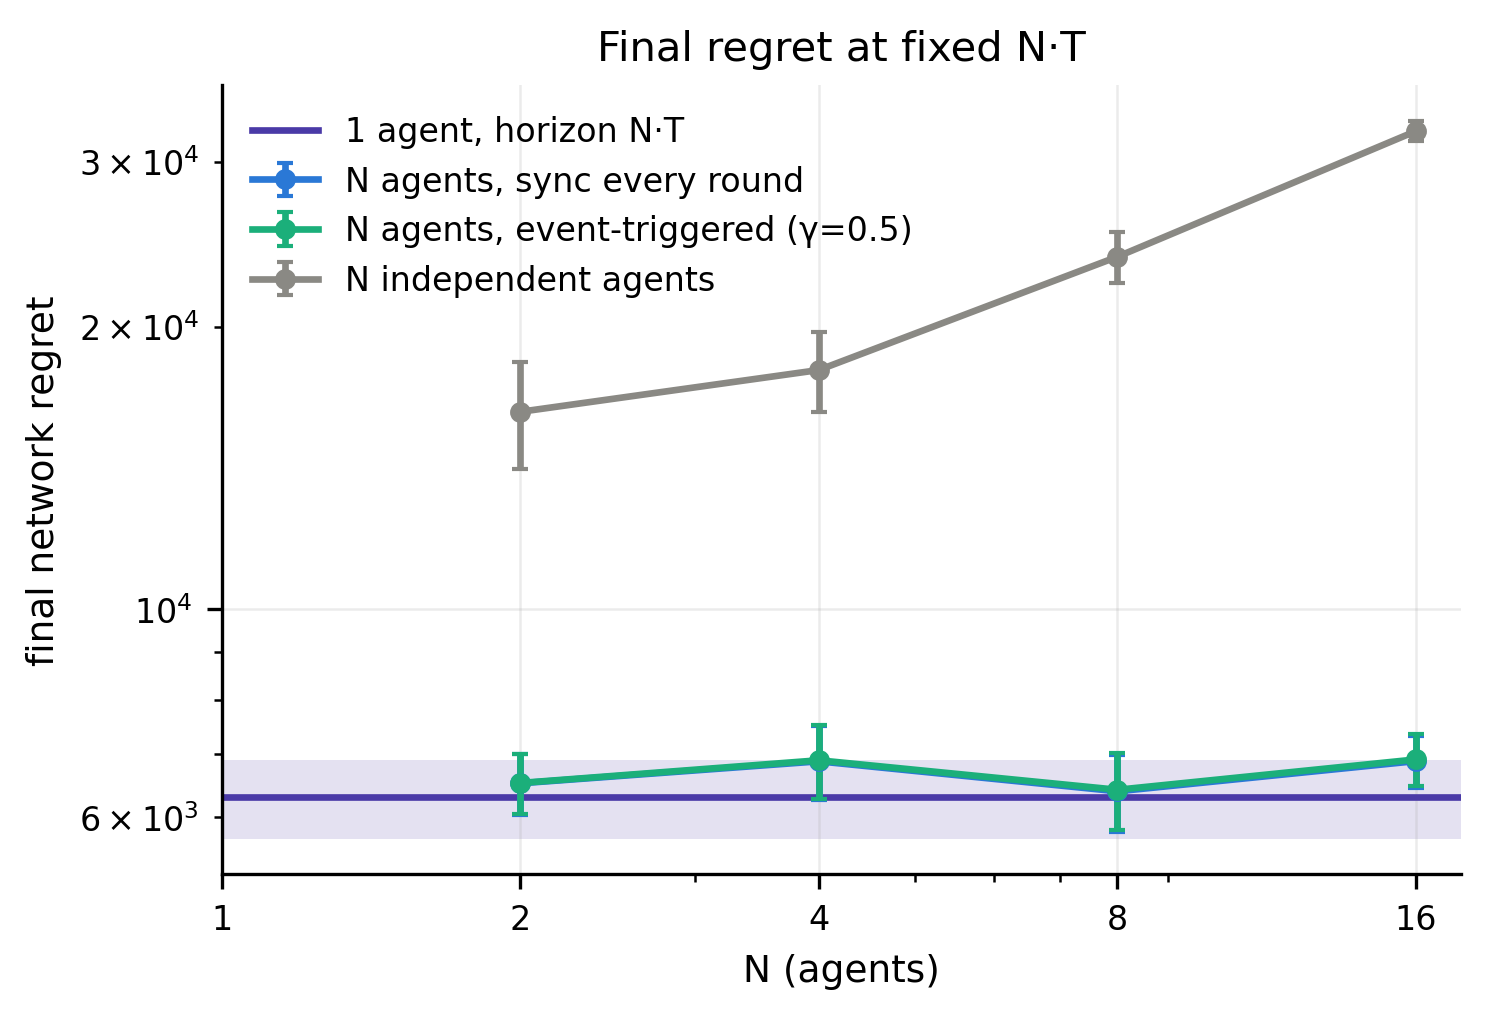
\includegraphics[width=\textwidth]{e22_vsN.png}\\
\centering\scriptsize E22: fixed budget $NT=160$k, 20 paired trials (quadratic link)
\end{column}
\begin{column}{0.48\textwidth}
\begin{itemize}
\item $N$ synced agents: within \textbf{0--10\%} of one agent at horizon $NT$, never better.
\item Independent agents: \textbf{2.3--5.1$\times$} worse.
\end{itemize}
\begin{block}{Proved (server)}
\textbf{Lower bound by simulation:} any $N$-agent algorithm $\ge c(NT)^{2/3}$.\\[0.2em]
\textbf{Upper bound:} Fed-ZoomSIB $=\tilde O\big((NT)^{2/3}\big)$.
\end{block}
\scriptsize The server rate is \emph{closed}, so it is the yardstick for the serverless version.
\end{column}
\end{columns}
\end{frame}

%====================================================================
\begin{frame}{Finding 3: what losing the server costs (E23)}
\small
\begin{columns}[c]
\begin{column}{0.5\textwidth}
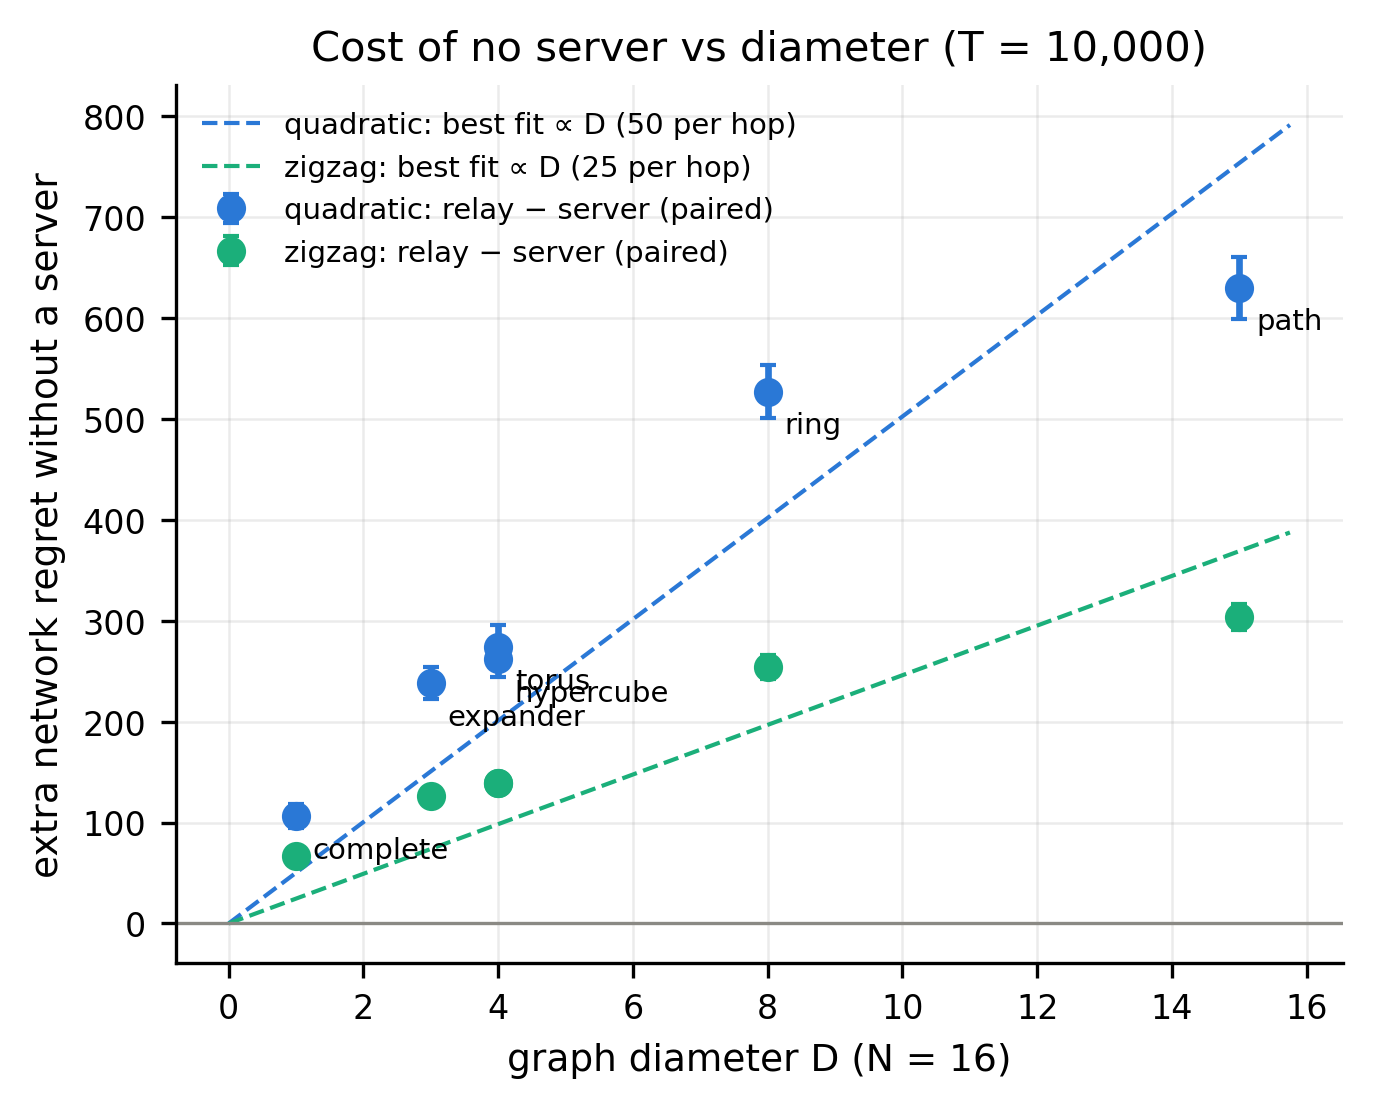
\includegraphics[width=\textwidth]{e23_vsD.png}
\end{column}
\begin{column}{0.5\textwidth}
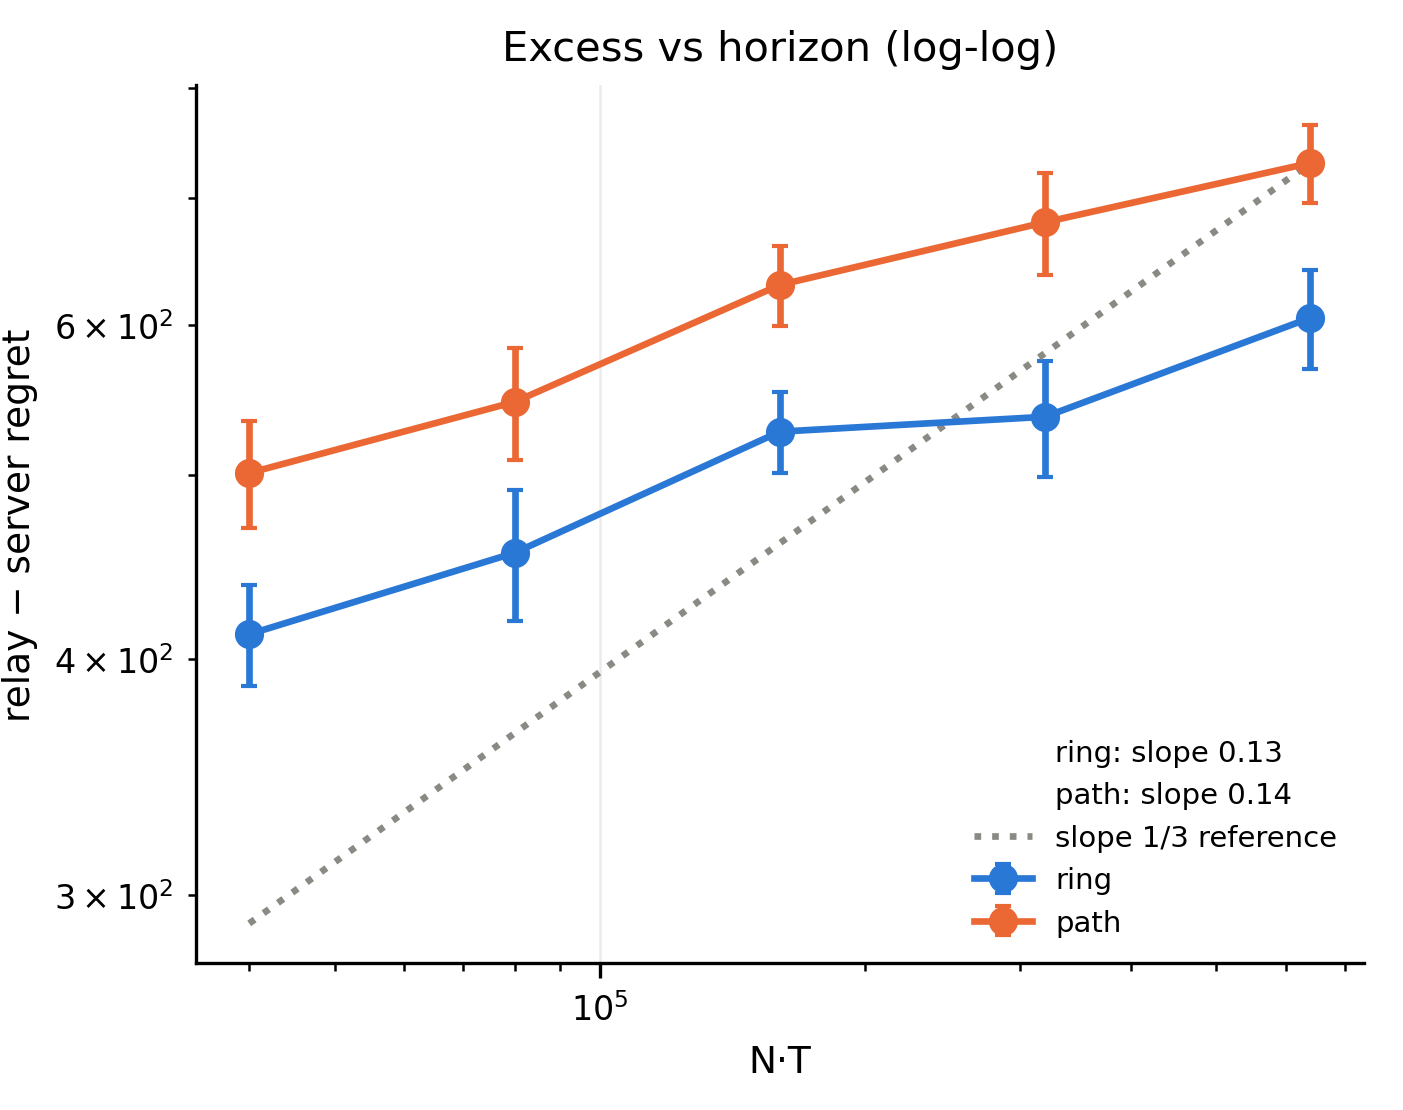
\includegraphics[width=\textwidth]{e23_vsT.png}
\end{column}
\end{columns}
\begin{itemize}
\item Extra regret: \textbf{+1.5\%} (complete, $D=1$) to \textbf{+9\%} (path, $D=15$), $N=16$; grows \emph{sublinearly} in $D$.
\item Nearly flat in the horizon: log-log slope \textbf{0.13--0.14} against the $1/3$ our bound predicts.
\item Relay sends 15--20\% \emph{fewer} scalars than the server (no broadcast to all $N$).
\end{itemize}
\end{frame}

%====================================================================
\begin{frame}{E32: delivery time, measured}
\small
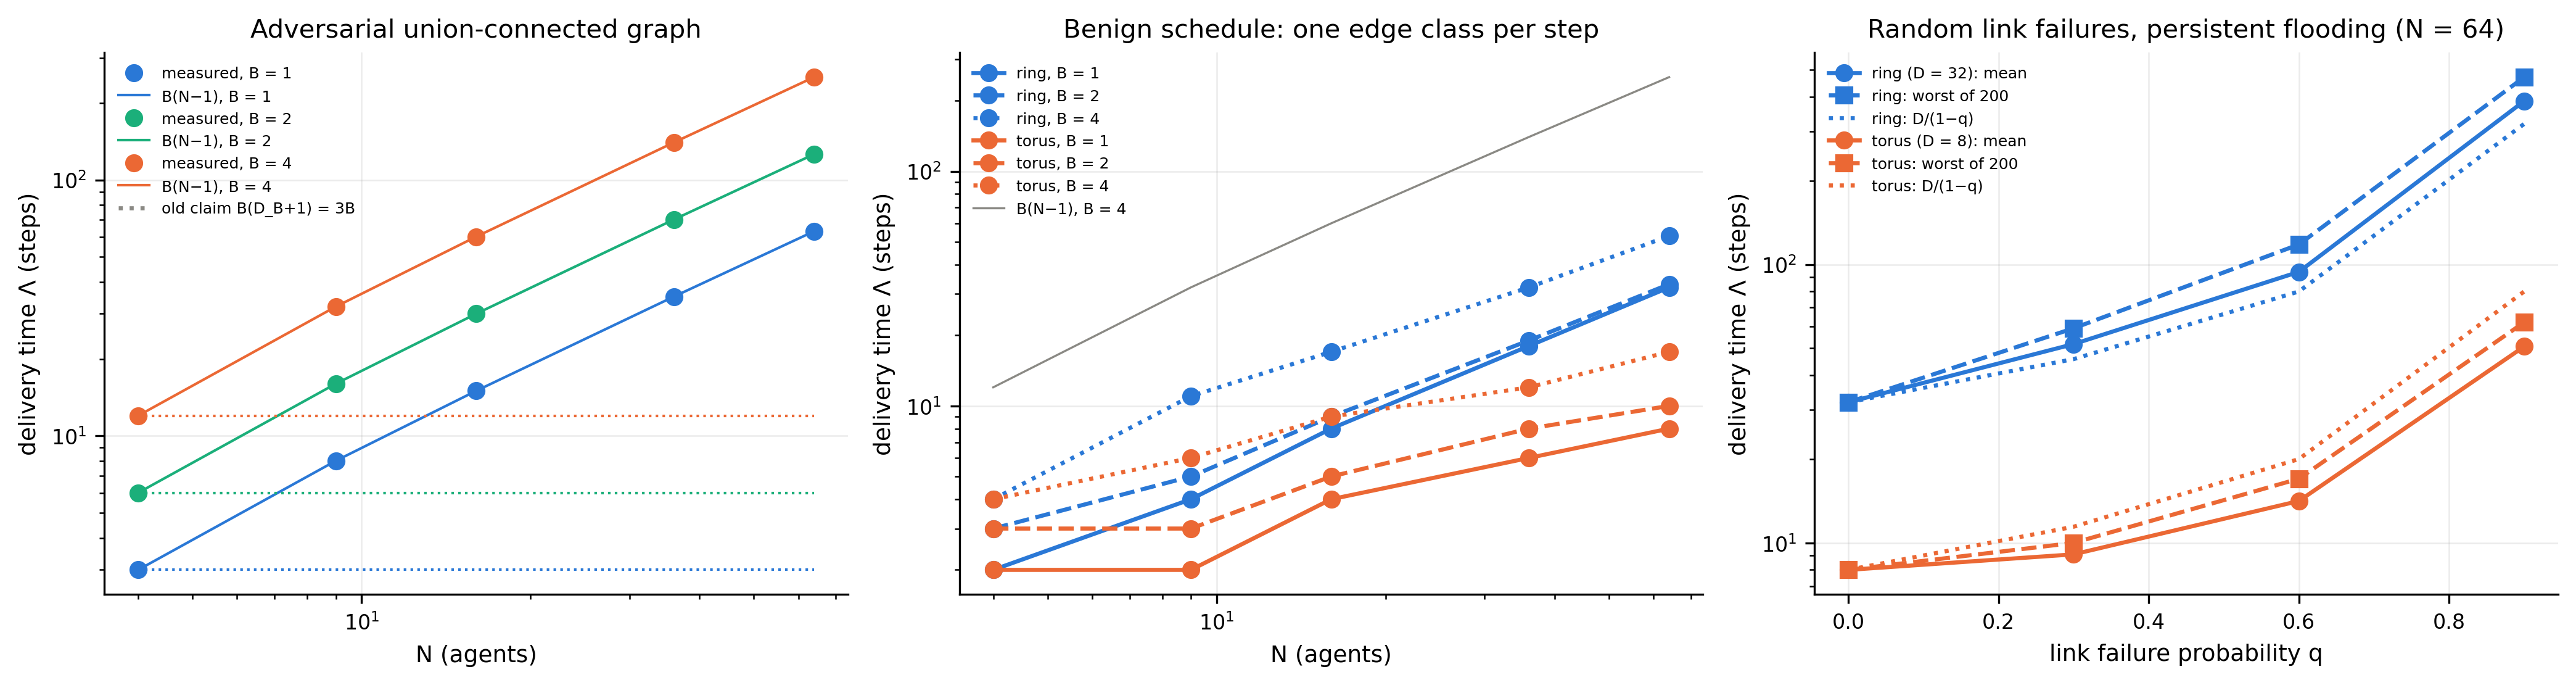
\includegraphics[width=\textwidth]{e32_delivery.png}
\begin{itemize}
\item \textbf{Adversarial star:} exactly $B(N-1)$ in every case; the old claim $3B$ is off by up to $21\times$ at $N=64$.
\item \textbf{Benign schedule} (one edge class per round): $\Lambda\le B\cdot D$, far below the worst case.
\item \textbf{Link failures:} worst of 200 runs within $1.5\times$ of $D/(1-q)$ (ring and torus, $N=64$).
\end{itemize}
\end{frame}

%====================================================================
\begin{frame}{Proposition 34: stopping Phase 1 without a server}
\scriptsize
\begin{block}{Proposition 34 (serverless stopping with agreement)}
At each fixed checkpoint every agent floods its local Stein sum. $\Lambda$ rounds later, every agent applies the \emph{server's} rule to the \emph{same} pooled sums. So all agents stop at the server's checkpoint and freeze the same $\hat\theta$ ($\eta_{\rm agree}=0$). Cost: $\le2L_fN\Lambda$ regret and $2|E|N(d{+}1)$ scalars per checkpoint.
\end{block}
\begin{columns}[c]
\begin{column}{0.52\textwidth}
\renewcommand{\arraystretch}{1.1}
\begin{tabular}{@{}lccc@{}}
\toprule
ring ($D=8$), E33 & stops at & disagree & $\div$ fixed\\
\midrule
fixed $T_0=60$ & 60 & 0 & 1.00\\
each agent, ``any'' & 24 & 0.058 & 1.67\\
each agent, ``all''$^*$ & 50 & 0.024 & 1.07\\
server rule & 28 & 0 & 1.34\\
\alert{pooled (Prop 34)} & \alert{36} & \alert{0} & 1.45\\
\bottomrule
\end{tabular}\\[0.2em]
{\tiny $^*$assumes detection is free. Tolerance 0.15; 0.05 gives the same picture.}
\end{column}
\begin{column}{0.46\textwidth}
\begin{itemize}
\item \textbf{Exactly as proved:} stops \emph{exactly} $D$ rounds after the server (4, 8, 15) in every one of 20 paired trials, with zero disagreement.
\item \textbf{But adaptive stopping itself loses} to a fixed $T_0$, even with a server ($\times1.3$--$1.4$). The drift rule is the weak point, not the graph.
\end{itemize}
\end{column}
\end{columns}
\end{frame}

%====================================================================
\begin{frame}{Theorem 35: a private Phase 1}
\scriptsize
\begin{columns}[c]
\begin{column}{0.55\textwidth}
\begin{block}{Theorem 35}
Each agent adds Gaussian noise once to its truncated Stein sum. Then everything the network does is $(\varepsilon,\delta)$-DP for every Phase-1 sample, and the direction error grows by a factor $1+\kappa$, with
\[
\kappa=\sqrt{6dN\log(1.25/\delta)}/\varepsilon .
\]
A longer Phase 1 buys it back: the leading term becomes $\tilde O\big(((1{+}\kappa)dNT)^{2/3}\big)$.
\end{block}
\end{column}
\begin{column}{0.43\textwidth}
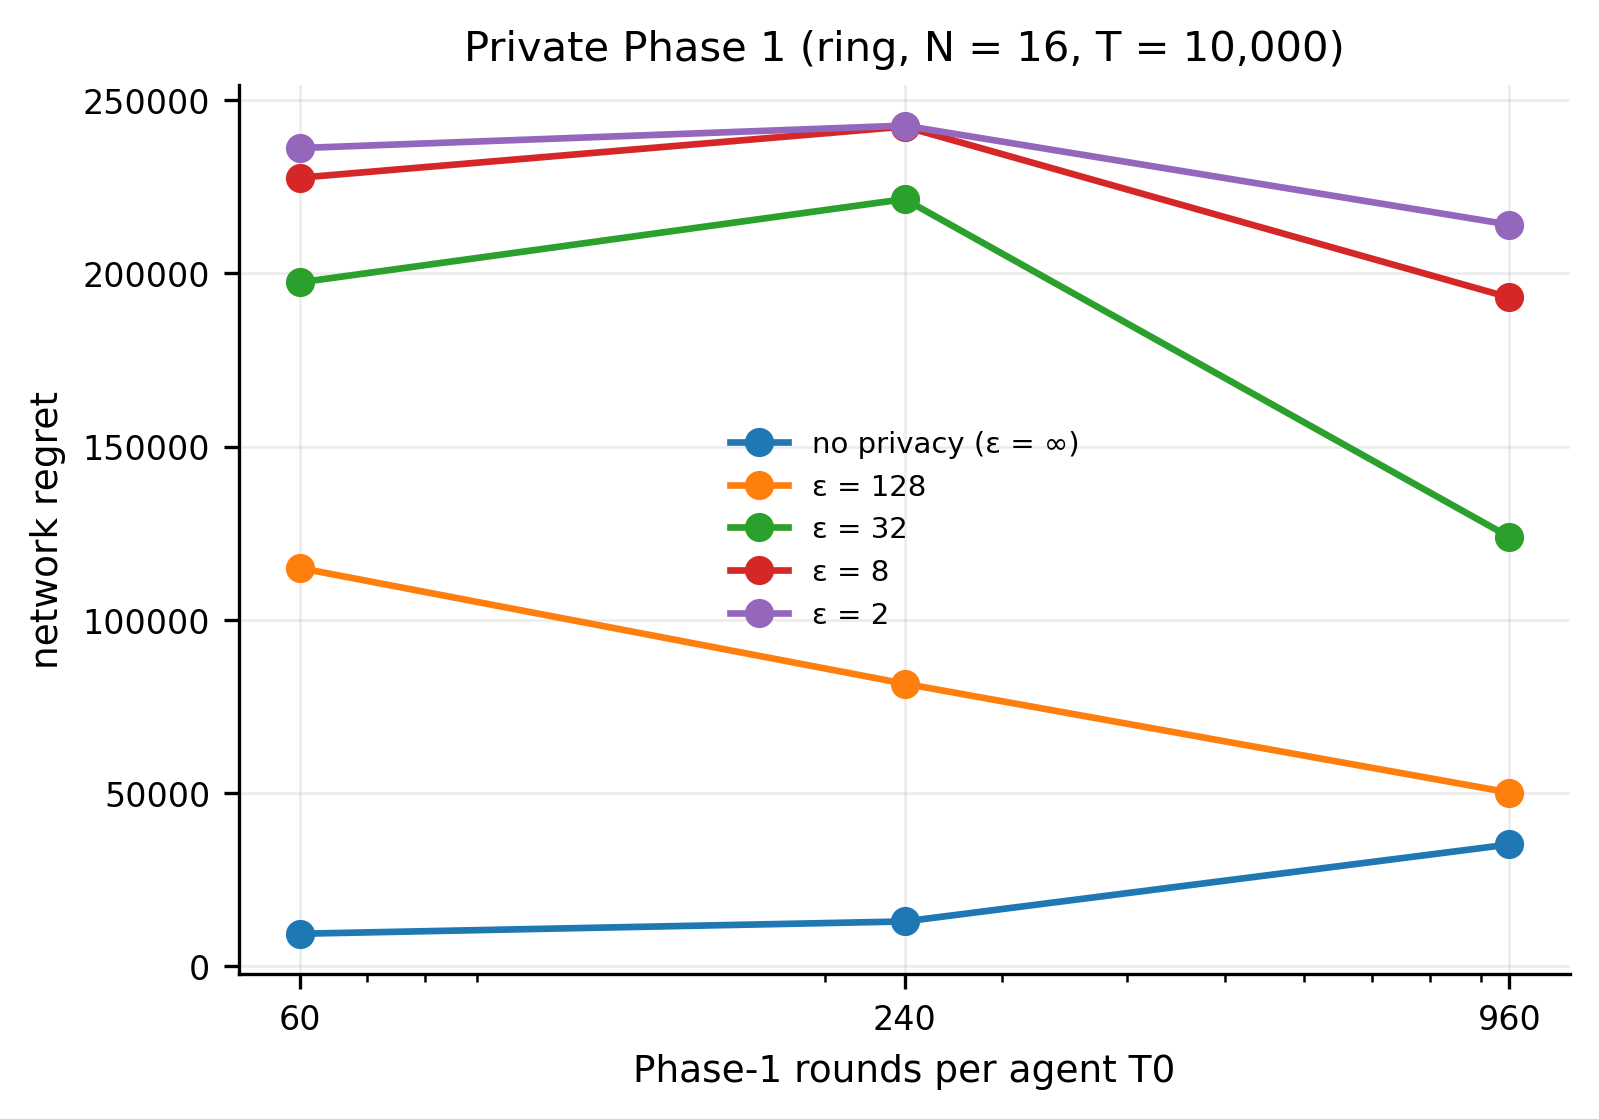
\includegraphics[width=\textwidth]{e35_private.png}
\end{column}
\end{columns}
\begin{alertblock}{E35: the constants make it impractical at our scale}
The noise scales with the worst-case truncation level ($L_f=48$ for the quadratic link), about $20\times$ a typical summand. $\varepsilon\le32$ gives a random direction. $\varepsilon=128$ costs $\times12$ at $T_0=60$ and $\times5$ at $T_0=960$: the trend the theorem predicts, but far from free.
\end{alertblock}
\textbf{Open:} a smaller clipping level (bias vs noise); private \emph{Phase 2}, where actions leak the agent's own rewards.
\end{frame}

%====================================================================
\begin{frame}{Checking the proofs: what changed}
\small
We re-checked every step against DBG's paper. Five changes:
\begin{enumerate}
\item \textbf{Noise:} DBG's Stein lemma (B.1) is proved for i.i.d.\ samples, but their assumption is only conditional sub-Gaussianity. We state i.i.d.\ noise explicitly.
\item \textbf{Hard instances:} DBG's lower bound uses $K\approx n^{1/3}\log n$ arms and $\mu^*\sim1/\log n$, not a fixed $K$. Our Theorem 5 states this class.
\item \textbf{Expectation vs high probability:} $f$ is bounded only near $0$, so the regret theorem is stated with high probability (as DBG do). It holds in expectation when $f$ is bounded, as on the hard instances.
\item \textbf{Time-varying graphs:} our first bound $B(D_B{+}1)$ was \alert{wrong}. The star example breaks it, and the correct bound is $B(N-1)$, which is tight (E32).
\item \textbf{Simpler trigger:} comparing with the latest epoch the agents already hold halves the epoch count: $|\mathcal E|\le1+N_b(1+\log_{1+\gamma}NT)$.
\end{enumerate}
\scriptsize Each point is logged with context in \texttt{docs/proofs/remarks.md} (R1--R11).
\end{frame}

%====================================================================
\begin{frame}{Finding 4: communication is all in Phase 2}
\small
\begin{columns}[c]
\begin{column}{0.5\textwidth}
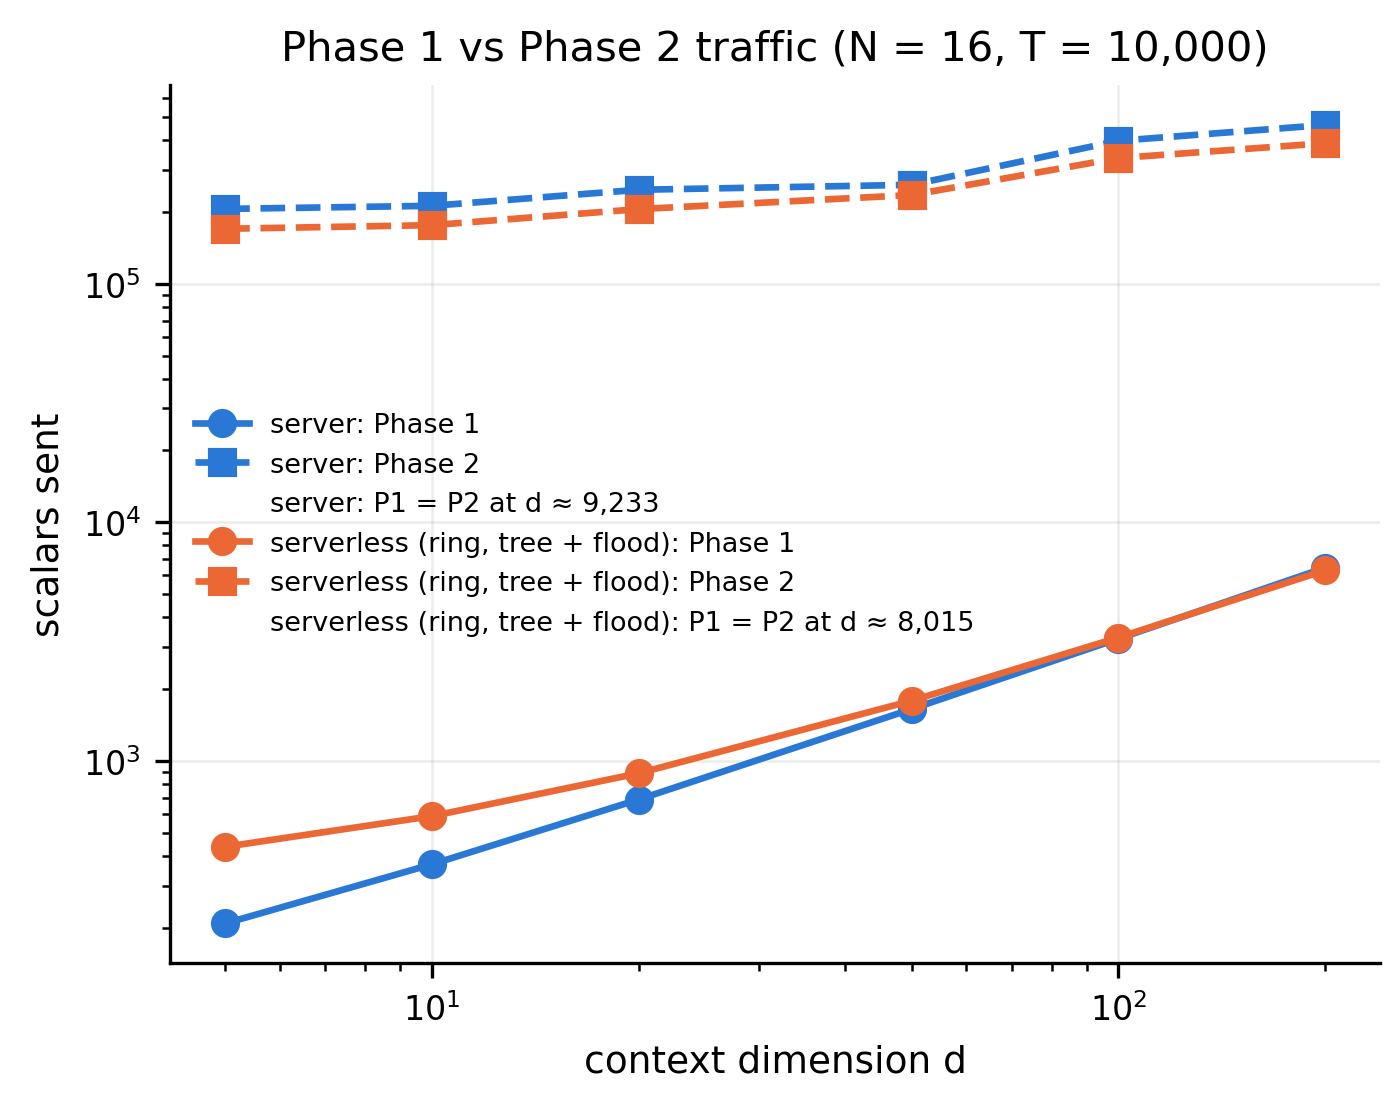
\includegraphics[width=\textwidth]{e24_traffic.png}
\end{column}
\begin{column}{0.5\textwidth}
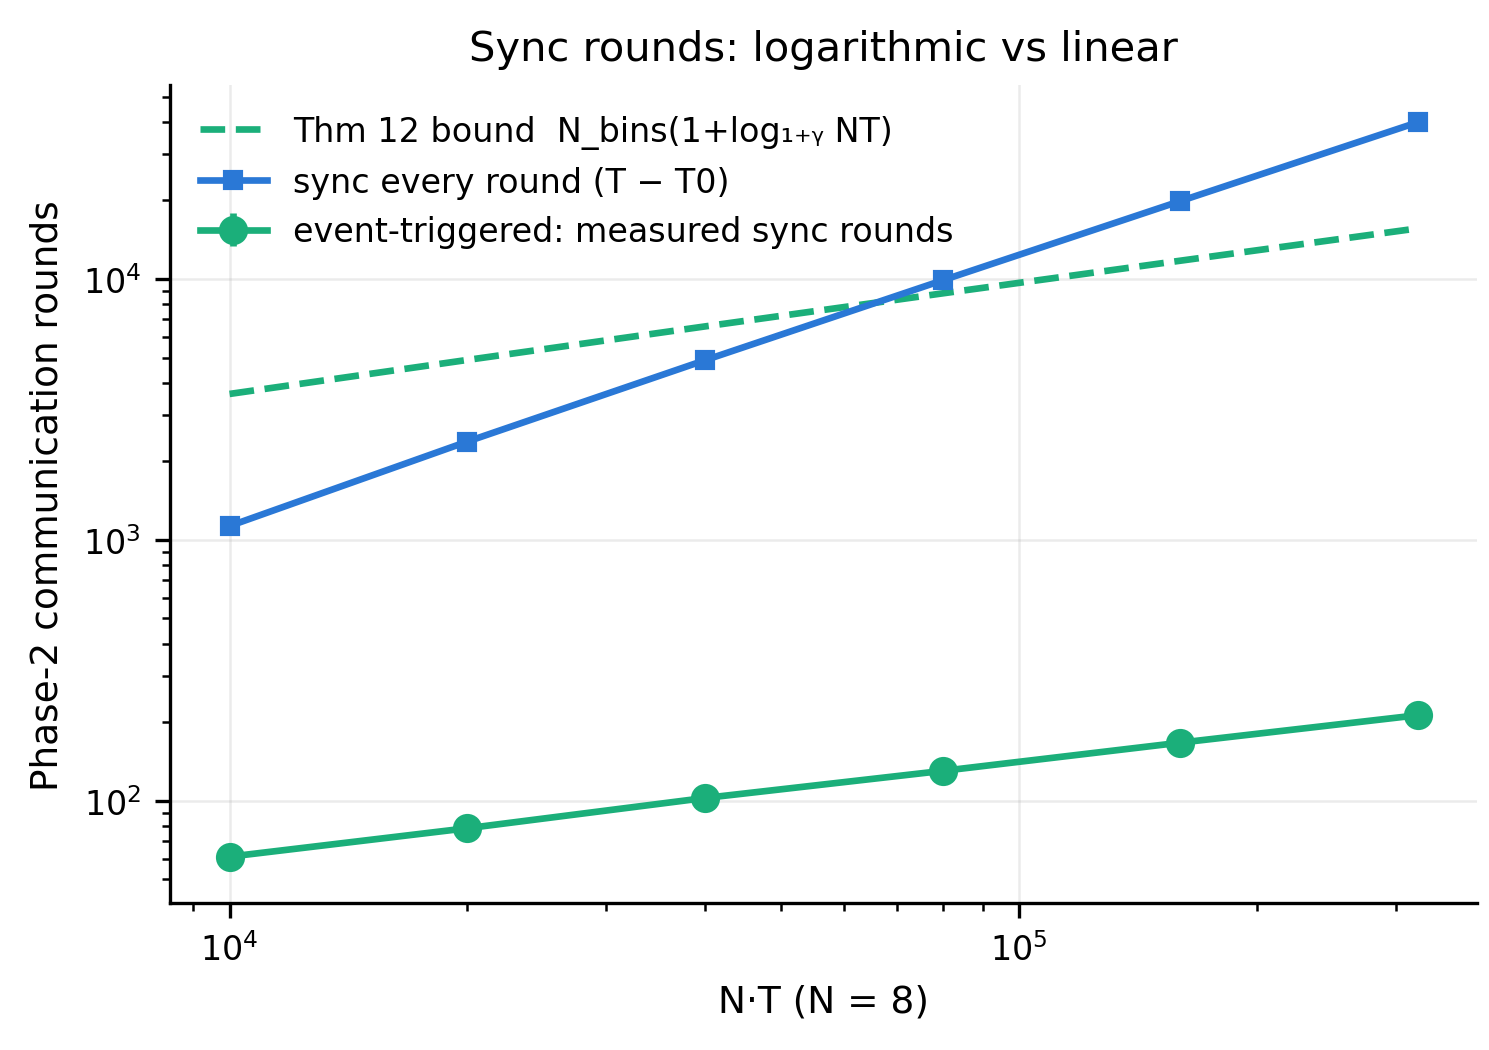
\includegraphics[width=\textwidth]{e22b_syncs.png}
\end{column}
\end{columns}
\begin{itemize}
\item Phase 1 is \textbf{0.1--1.6\%} of all traffic ($d=5\ldots200$), and shrinks with $NT$; compressing it saves $\le0.4\%$ of bits.
\item Event-triggered sync: 61$\to$213 rounds as $NT$ grows $32\times$ (per-round sync: 1k$\to$40k), at the same regret.
\end{itemize}
\end{frame}

%====================================================================
\begin{frame}{Finding 5: agents must agree, not explore longer}
\small
\begin{columns}[c]
\begin{column}{0.5\textwidth}
\centering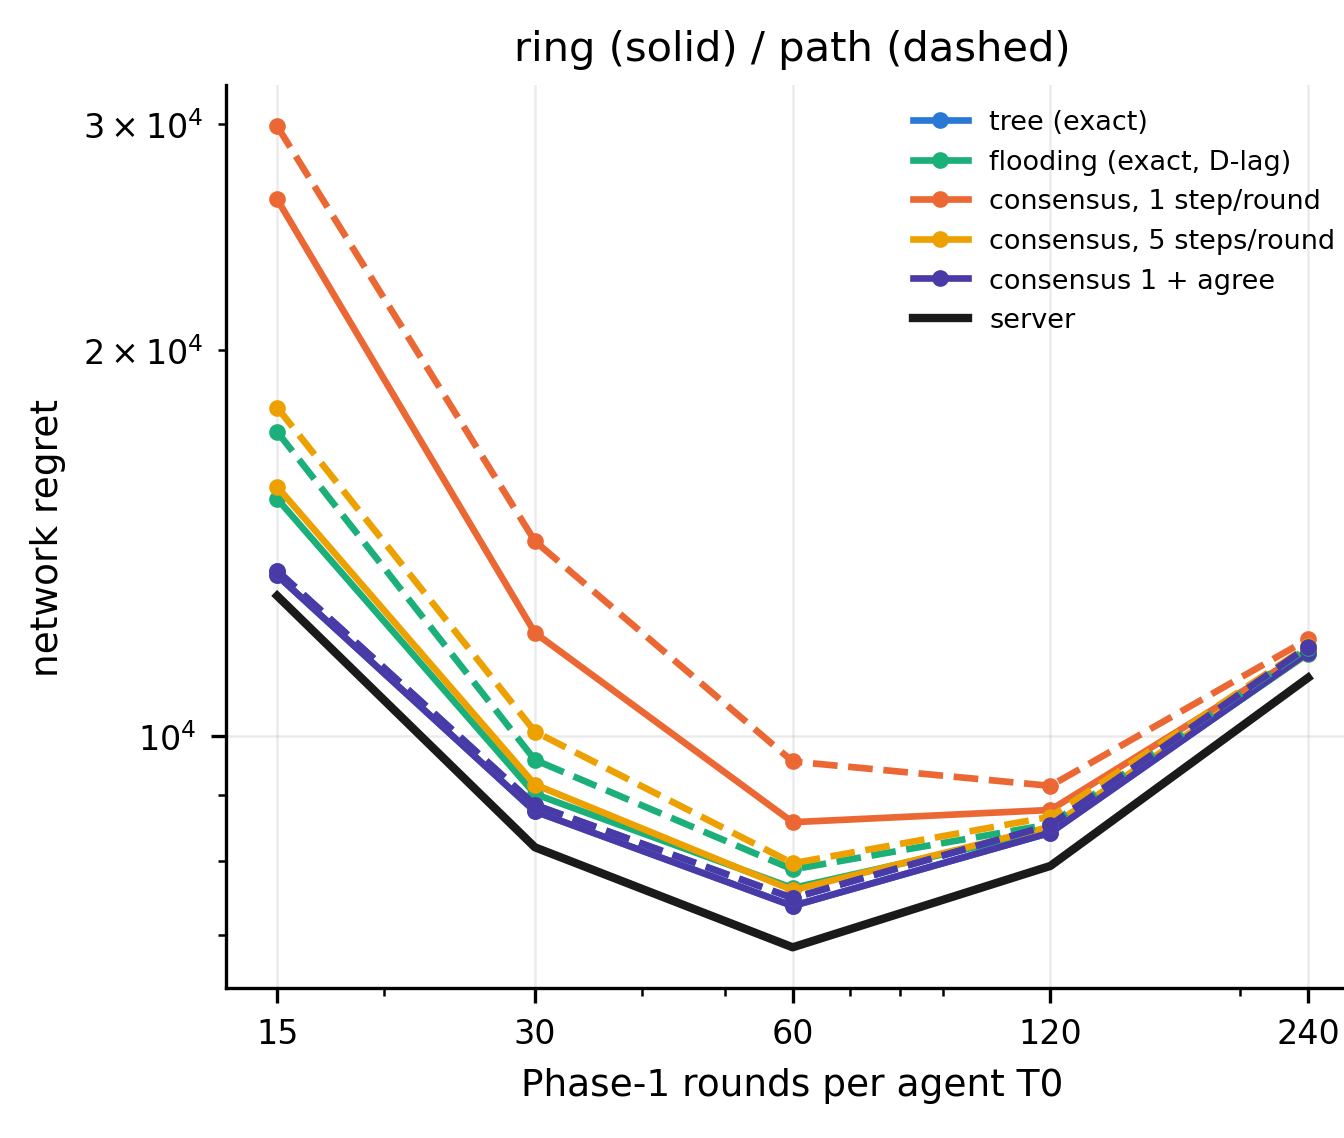
\includegraphics[width=0.9\textwidth]{e28_T0.png}
\end{column}
\begin{column}{0.5\textwidth}
\centering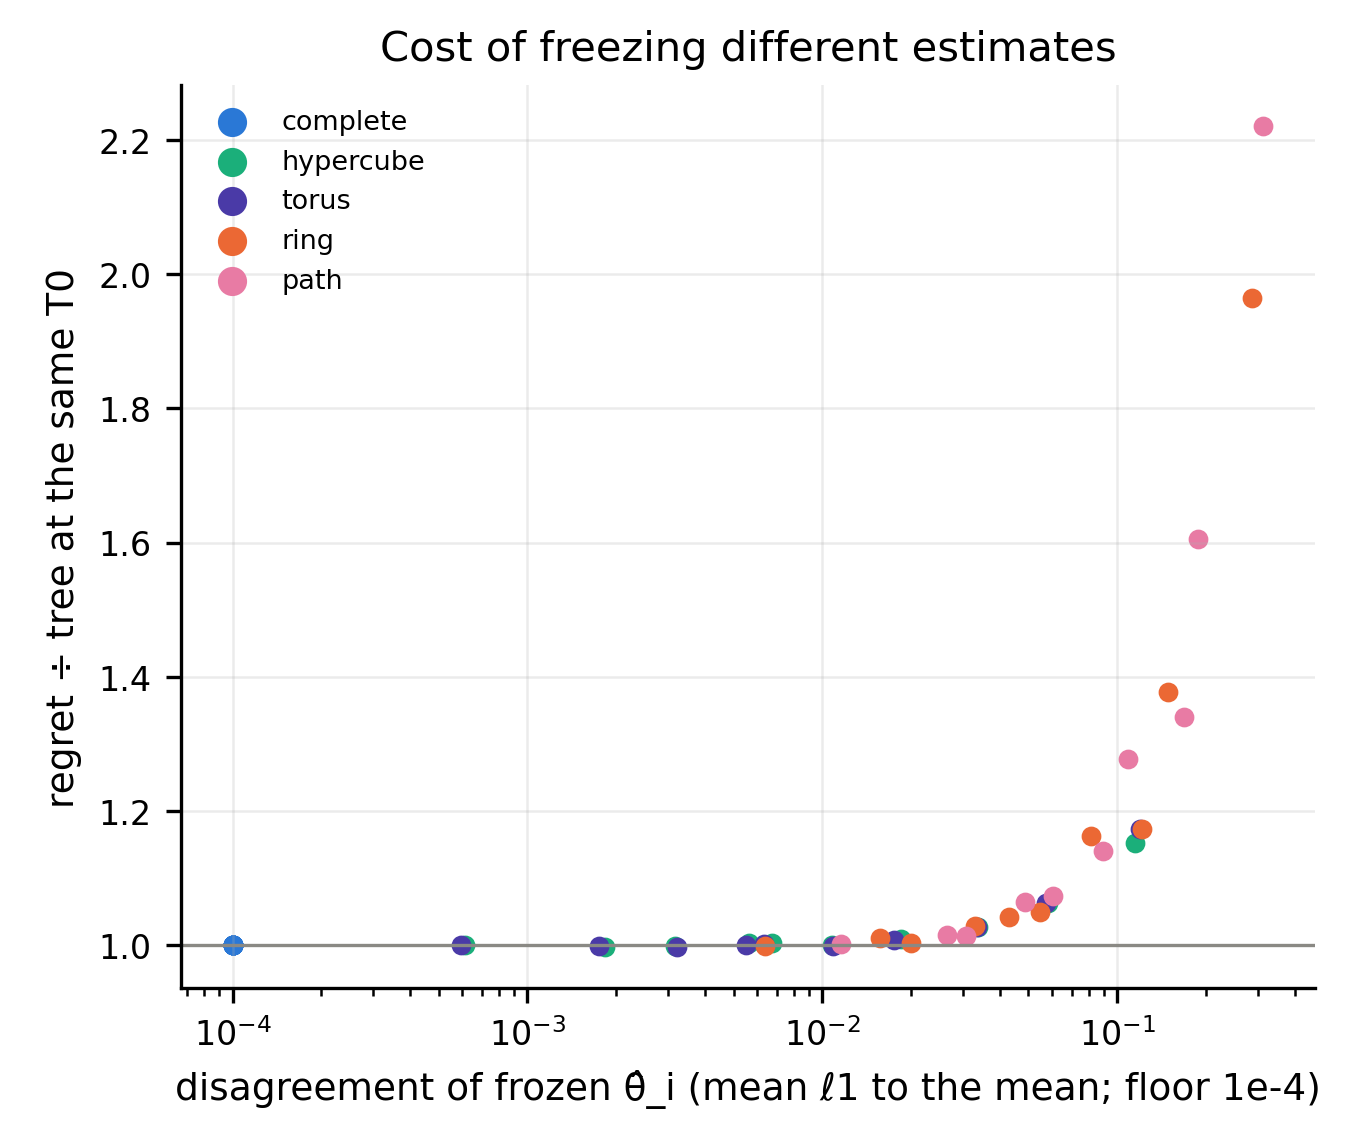
\includegraphics[width=0.9\textwidth]{e28_disagree.png}
\end{column}
\end{columns}
\begin{itemize}
\item The best exploration length $T_0^*$ barely moves with the graph.
\item The cost is agents freezing \emph{different} $\hat\theta_i$: consensus costs $\times$1.25 (ring), $\times$1.34 (path).
\item \textbf{One agreement pass} at the freeze removes it, for $\sim$2.8k extra scalars.
\end{itemize}
\end{frame}

%====================================================================
\begin{frame}{Finding 5: adaptive stopping on graphs fails}
\small
\begin{columns}[c]
\begin{column}{0.56\textwidth}
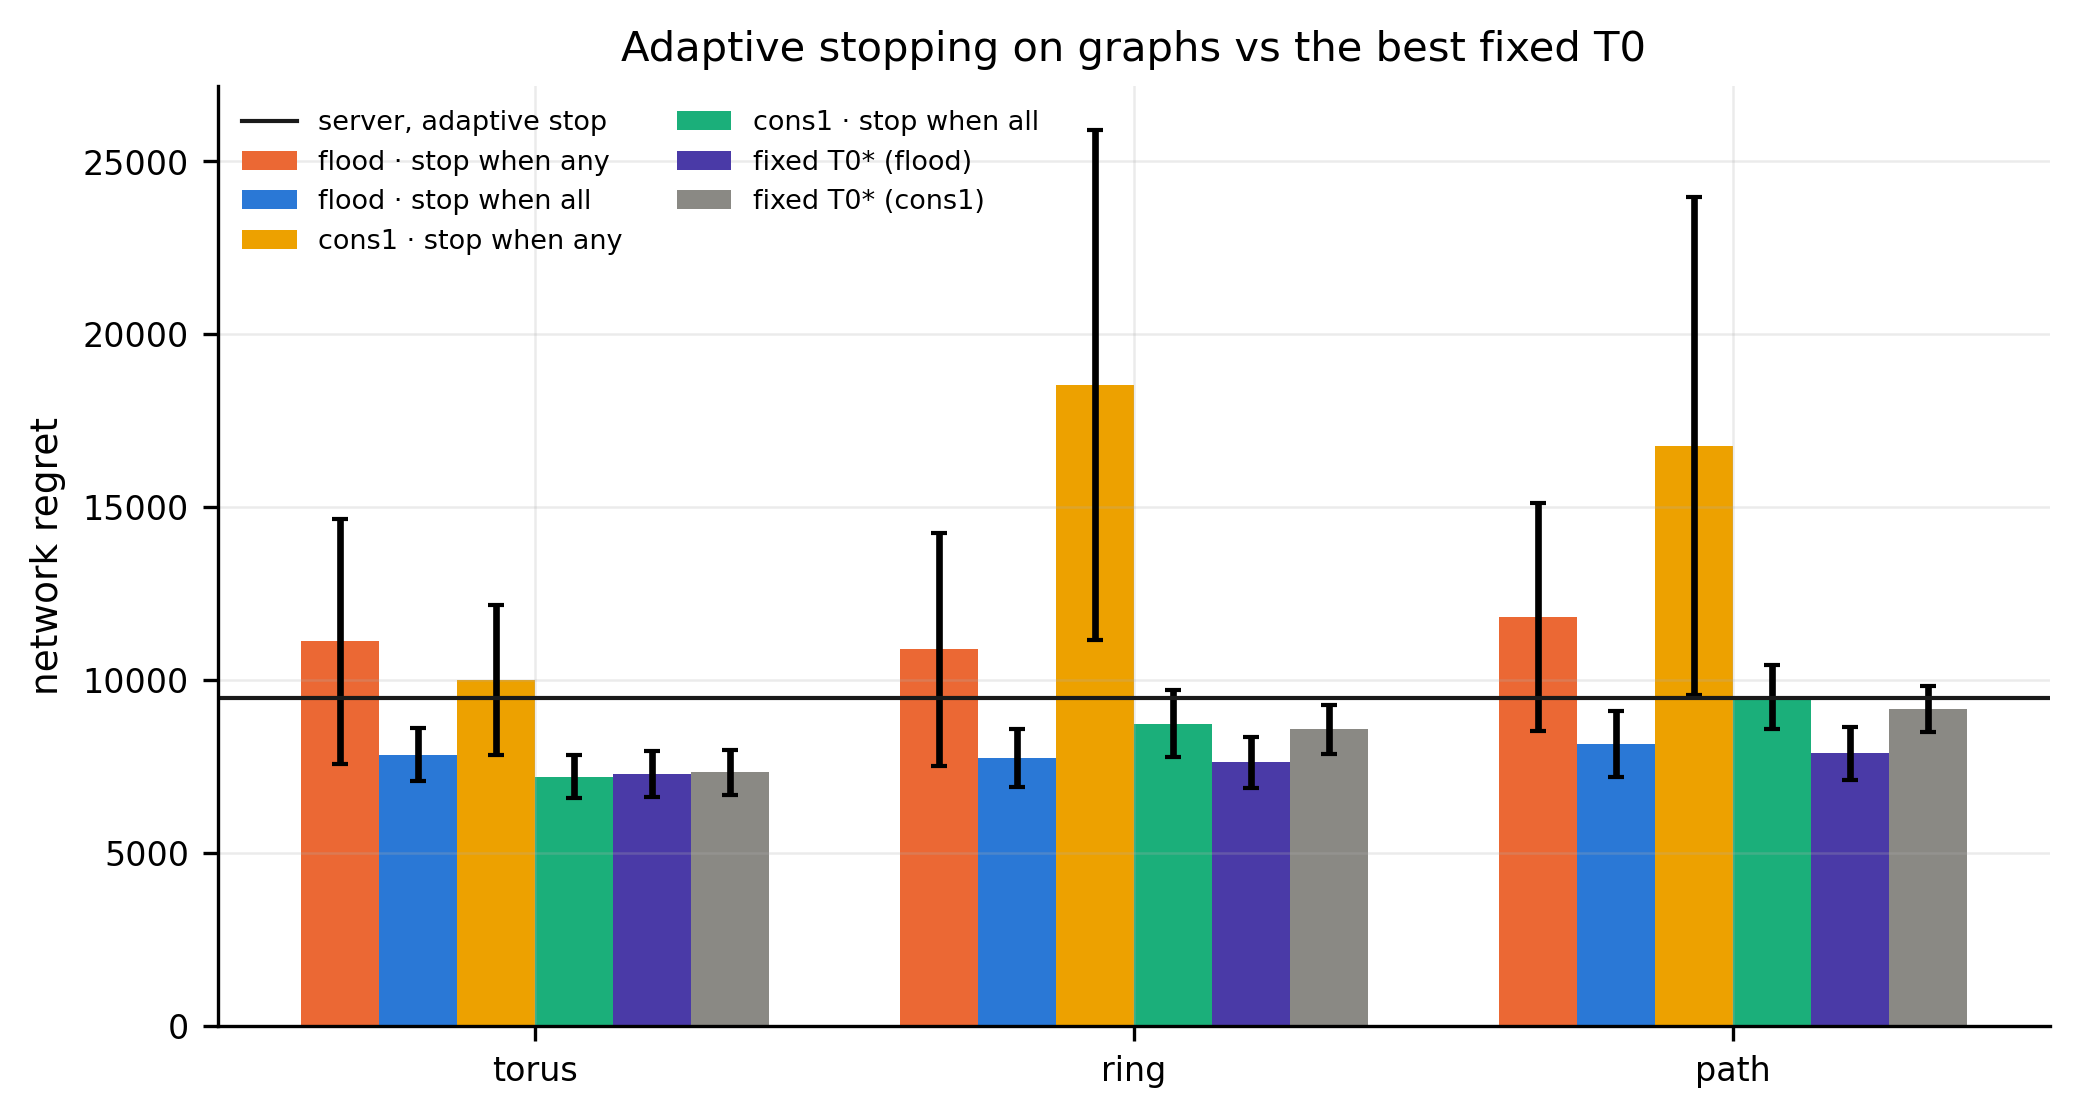
\includegraphics[width=\textwidth]{e28b_stop.png}
\end{column}
\begin{column}{0.42\textwidth}
\begin{itemize}
\item ``Stop when \emph{any} agent is stable'': \textbf{1.4--2.2$\times$} regret, high variance.
\item ``Stop when \emph{all} are'': close to fixed $T_0$, but needs $\ge D$ extra rounds to detect (not modelled).
\item Even the server's adaptive stop is worse than a fixed $T_0$.
\end{itemize}
\begin{block}{Now answered (Prop 34)}
Apply the server's rule to flooded pooled sums: exact agreement, $\Lambda$ rounds later.
\end{block}
\end{column}
\end{columns}
\end{frame}

%====================================================================
\begin{frame}{Summary of findings}
\tiny
\renewcommand{\arraystretch}{1.15}
\begin{tabular}{>{\raggedright\arraybackslash}p{4.6cm}>{\raggedright\arraybackslash}p{5.6cm}}
\toprule
\textbf{Claim} & \textbf{Evidence}\\
\midrule
Collaboration pays without a server & regret $\propto N^{0.44\text{--}0.55}$ vs $N^{0.98}$ alone (E19)\\
Relaying: same regret, far less talk & $\times$1.03 of server at its communication; mixing needs $\sim2000\times$ more scalars (E15, E20)\\
Robust to failing links & +27\% at 90\% link failures (E18)\\
Server = one agent at $NT$ & within 0--10\%; proved lower + upper bound (E22)\\
No server costs little & +1.5\% to +9\%, nearly flat in $T$ (E23)\\
Graph cost has the proved shape & epochs: excess $/NDK=0.86$--$1.15$; relays: excess $\propto$ farness; flat in $T$ (E31, E36)\\
Provable relay beats the relay we ran & lower excess on every graph, $7$--$8\times$ more scalars (E36)\\
Dependence on $K$ & grows like $K^{0.4}$--$K^{0.5}$; bounds are linear in $K$ (E36)\\
Communication is Phase 2 & Phase 1 $<2\%$; logarithmic sync rounds (E22, E24)\\
Agreement is what matters & disagreement $\times$1.25--1.34, fixed by one pass (E28); stopping with agreement (E33)\\
Delivery time on time-varying graphs & $B(N-1)$ is tight; benign schedules far below (E32)\\
Prior algorithms on our problem & best on non-monotone links, gap grows with $T$; monotone methods win on monotone links (E34)\\
Private Phase 1 & provable but costly at our scale (E35)\\
\bottomrule
\end{tabular}
\end{frame}

%====================================================================
\begin{frame}{Baselines for the serverless setting}
\small
\begin{block}{1. Reference baselines (as in DLUCB, Coop-KernelUCB)}
No communication (independent ZoomSIB) \quad and \quad centralised (server) \hfill \yes\ done
\end{block}
\begin{block}{2. Prior papers' protocols, run with ZoomSIB}
Running consensus (Landgren et al.), gossip (DDUCB), accelerated consensus (DLUCB), message passing (Coop-Kernel), push-sum \hfill \yes\ done
\end{block}
\begin{block}{3. Prior papers' algorithms, run on our problems}
\begin{itemize}
\item DLUCB-style (LinUCB), Dec-ESTOR, Dec-GSTOR, Coop-Kernel-style (IGP-UCB), each with \emph{ideal} relaying of all raw data \hfill \yes\ done (E34)
\end{itemize}
\end{block}
\end{frame}

%====================================================================
\begin{frame}{Status and next steps (Paper A)}
\tiny
\renewcommand{\arraystretch}{0.95}
\begin{tabular}{>{\raggedright\arraybackslash}p{5.3cm}>{\raggedright\arraybackslash}p{4.1cm}c}
\toprule
\textbf{Work} & \textbf{Deliverable} & \textbf{Status}\\
\midrule
Server theorem: lower + upper bound & \texttt{docs/proofs/server.pdf} & \yes\\
Relay theorem (synchronised epochs) & Thm 17, Cor 18 & \yes\\
Communication, bounded memory & Thm 29, Prop 30 & \yes\\
Directed / delayed / time-varying / failing links & Lemma 31, Cor 32; E32 & \yes\\
Agreement; stopping with agreement & Thm 33, Prop 34; E28, E33 & \yes\\
Proved vs run protocol; trigger cost & E31 & \yes\\
Prior algorithms on our problem & E34 & \yes\\
\midrule
Delay term: horizon-free, matches E31 shape & Thm 22; E31, E36 & \yes\\
A provable relay as good as the one we ran & Thm 27; E36 & \yes\\
Graph lower bound $\Omega(N\min(T,D)^{1/3})$ & Thm 7, Cor 8 & \yes\\
Upper $KF'$ vs lower $ND^{1/3}$: close the gap & open problem & \todo\\
Privacy & Thm 35: Phase 1 only, costly (E35) & \textcolor{orange!85!black}{partly}\\
\midrule

Related-work section; write-up & AISTATS-style draft & \todo\\
\bottomrule
\end{tabular}
\vspace{0.1em}
\begin{center}
\fbox{\parbox{0.9\textwidth}{\centering\footnotesize\textbf{Paper A:} the first single-index bandit over a network: optimal with a server, and what the graph costs without one.}}
\end{center}
\end{frame}

\end{document}
